\section{Methods}

\subsection{Data}

Data was used for all emergency stroke admissions to England and Wales for the 5 years 2017-2021, for teams with average admissions of at least 250 admissions over the 5 years. The total number of patients were, 302,715, of whom 114,625 (38\%) arrived within 4 hours of known stroke onset. Of those arriving within 4 hours of known stroke onset 103,244 (90\%) arrived by ambulance.

The following data fields from SSNAP were used in the modelling:

\begin{itemize}

    \item \textit{Stroke team}: Stroke team attended (hospital identifier).

    \item \textit{Age}: As midpoint of 5 year age bands.

    \item \textit{Sex}.

    \item \textit{Diagnosis of atrial fibrillation}: Did the patient have a diagnosis of atrial fibrillation, either made prior to admission, or during admission?

    \item \textit{Use of anticoagulants}: Use of prior anticoagulant for atrial fibrillation.

    \item \textit{Onset known}: Whether onset was known, and if known whether it was considered to be known precisely or was a best estimate.

    \item \textit{Onset during sleep}: Did stroke occur in sleep? (1 = Yes, 0 = No).

    \item \textit{Onset-to-arrival time}: Time from onset of stroke to arrival at hospital (minutes), when known.

    \item \textit{Prior disability level}: Estimated modified Rankin Scale, mRS, prior to stroke.

    \item \textit{Stroke type}: Infarction/haemorrhage.

    \item \textit{Stroke severity}: National Institutes of Health Stroke Scale (NIHSS) score on arrival.

    \item \textit{Arrival-to-scan time}: Time from arrival at hospital to scan (minutes), when known.

    \item \textit{Scan-to-thrombolysis time}: Time from arrival at hospital to scan to treatment with thrombolysis  (minutes), when given.
    
\end{itemize}

\subsection{Overview}

Figure \ref{fig:flow} shows an overview of the process steps included in the modelling. The steps were:

\begin{enumerate}

    \item \textit{Stroke onset}: 

    \item 
    
\end{enumerate}


\begin{figure}
    \centering
    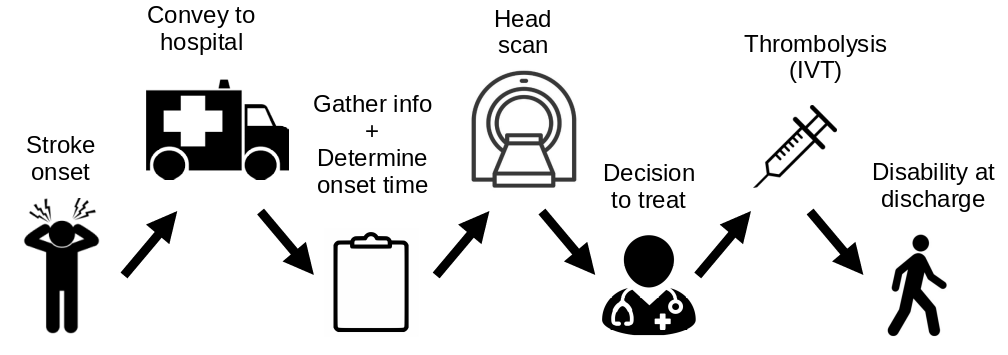
\includegraphics[width=0.75\linewidth]{images/flow}
    \caption{An overview of the process steps included in the modelling.}
    \label{fig:flow}
\end{figure}



\subsection{Thrombolysis decision model}

The thrombolysis decision model has been described in more detail previously \cite{pearn_what_2023}. Feature selection was used to identify 10 key features that were most predictive of whether thrombolysis was used in any given stroke team. The model uses XGBoost \cite{chen_xgboost_2016} for predictions, and SHAP \cite{lundberg_unified_2017} for local (patient-level) and global (model/population-level) explainability. SHAP values show the contribution of each feature value to the final model predictions.

The thrombolysis decision model was applied only to patients arriving within 4 hours of known stroke onset (stroke onset was known precisely or was a best estimate). The 10 features used for predicting thrombolysis use were: Stroke team; Age; Precisely known onset time; Onset during sleep; Onset-to-arrival time; Arrival-to-scan time; Stroke type; Stroke severity; Prior disability level; Use of anticoagulants.

\subsubsection{Prototype patients}

To help compare decision-making and outcomes across stroke teams we exemplified differences using \textit{prototype patients}. These prototype patients captured a range of features known to affect decisions to treat, and to affect outcomes, and included an \textit{ideal} candidate for thrombolysis. The prototype patients used were:

\begin{enumerate}
    \item \textit{Ideal}: Onset-to-arrival = 90 minutes; arrival-to-scan = 15 minutes; onset-to-thrombolysis = 120 minutes; stroke severity (NIHSS) = 15; pre-stroke disability (mRS) = 0; age = 72.5; Precisely known onset; onset not during sleep; stroke type = Infarction; patient has no atrial fibrillation and is not receiving anticoagulants for atrial fibrillation.

    \item \textit{Late arrival}: as \textit{ideal} but onset-to-arrival = 225 minutes and onset-to-thrombolysis (when given) = 255 minutes.

    \item \textit{Mild}: As \textit{ideal} but stroke severity = 3.

    \item \textit{Prior disability}: as \textit{ideal} but pre-stroke disability = 3

    \item \textit{Imprecise}: as \textit{ideal} but stroke onset time estimated.

    \item \textit{Age}: as \textit{ideal} but age = 87.5.

    \item Combinations of the above.
\end{enumerate}

\subsubsection{Benchmark stroke teams and benchmark decisions}

SHAP isolates the contributes of features to model predictions. As one feature is the stroke team, the stroke team SHAP shows the influence of attending that stroke team on the likelihood of a patient receiving thrombolysis. Averaging stroke team SHAP values for all patients attending a given hospital provided a measure of the overall willingness of that stroke team to use thrombolysis (or how much that stroke team affected the odds of a patient receiving thrombolysis in the model). We took the stroke teams with the 25 highest stroke team SHAP values as \textit{benchmark stroke teams}. For any given patient, predictions can be made about whether each of the stroke teams would, or would not, give that patient thrombolysis. We took a majority vote of those 25 decisions as a \textit{benchmark decision} for that patient.

\subsection{Stroke outcome machine learning model}

\subsection{Lifetime economic model}

\subsection{Pathway model}

\subsection{Code and artificial patients}